\documentclass{article}

\usepackage[utf8]{inputenc}
\usepackage{amsthm}
\usepackage{amssymb}
\usepackage{mathtools}
\usepackage{graphicx}
\usepackage{mdframed}
\usepackage{float}
\usepackage[top=0.75in, bottom=0.75in, left=0.75in, right=0.75in]{geometry}
\usepackage{gauss}

\usepackage{array}
\allowdisplaybreaks

\makeatletter
\newcounter{elimination@steps}
\newcolumntype{R}[1]{>{\raggedleft\arraybackslash$}p{#1}<{$}}
\def\elimination@num@rights{}
\def\elimination@num@variables{}
\def\elimination@col@width{}
\newenvironment{elimination}[4][0]
{
    \setcounter{elimination@steps}{0}
    \def\elimination@num@rights{#1}
    \def\elimination@num@variables{#2}
    \def\elimination@col@width{#3}
    \renewcommand{\arraystretch}{#4}
    \start@align\@ne\st@rredtrue\m@ne
}
{
    \endalign
    \ignorespacesafterend
}
\newcommand{\step}[2]
{
    \ifnum\value{elimination@steps}>0\sim\quad\fi
    \left[
        \ifnum\elimination@num@rights>0
            \begin{array}
            {@{}*{\elimination@num@variables}{R{\elimination@col@width}}
            |@{}*{\elimination@num@rights}{R{\elimination@col@width}}}
        \else
            \begin{array}
            {@{}*{\elimination@num@variables}{R{\elimination@col@width}}}
        \fi
            #1
        \end{array}
    \right]
    & 
    \begin{array}{l}
        #2
    \end{array}
    \addtocounter{elimination@steps}{1}
}
\makeatother

\DeclarePairedDelimiter{\abs}{\lvert}{\rvert}
\DeclarePairedDelimiter{\norm}{\lvert \lvert}{\rvert \rvert}

\newtheoremstyle{break}% name
  {}%         Space above, empty = `usual value'
  {}%         Space below
  {\itshape}% Body font
  {}%         Indent amount (empty = no indent, \parindent = para indent)
  {\bfseries}% Thm head font
  {.}%        Punctuation after thm head
  {\newline}% Space after thm head: \newline = linebreak
  {}%         Thm head spec

\newtheorem{Def}{Definition}[section]

\theoremstyle{break}

\newtheorem{innerEx}{Exempel}[section]
\newtheorem{sats}{Sats}[section]
\newtheorem{Rem}{Anmärkning}[]

\newenvironment{Ex}
{\begin{mdframed} \begin{innerEx} \vspace{3pt}}
{\vspace{3pt} \end{innerEx} \end{mdframed}}  

\newenvironment{bevis}
{\begin{mdframed} \begin{proof} \vspace{3pt}}
{\vspace{3pt} \end{proof} \end{mdframed}}

\title{
	 Linjär Algebra\\
	 Föreläsning 9
    \author{Erik Sjöström}
}
\begin{document}
\maketitle
\section{$\mathbb{R}^n$} % (fold)
\label{sec:_r_n_}
En vektor i $\mathbb{R}^n$ är en n-tupel av reella tal:
\[
    \vec{u} = \begin{bmatrix} u_1\\u_2\\\vdots\\u_n \end{bmatrix}
\]
\begin{Rem}
    Man låter det vara en kolumnvektor av praktiska skäl
\end{Rem}
\noindent
Vektorer i $\mathbb{R}^2$ och $\mathbb{R}^3$ kan uppfattas som punkter eller vektorer i planet respektive rummet. Där vi utgår från en ON-bas.\\
Längden av $\vec{u}$:
\[
    \norm{\vec{u}} = \sqrt{u_1^2 + u_2^2 + \cdots + u_n^2}
\]
Addition, och multiplikation med skalär sker komponentvis:
\begin{align*}
&\vec{u} + \vec{v} = \begin{bmatrix} u_1\\\vdots\\u_n \end{bmatrix} + \begin{bmatrix} u_1\\\vdots\\_n \end{bmatrix} = \begin{bmatrix} u_1 + v_1\\\vdots\\u_n + v_n \end{bmatrix}
&& c \cdot \vec{v} = c \cdot \begin{bmatrix} v_1\\\vdots\\v_n \end{bmatrix} = \begin{bmatrix} c \cdot v_1\\\vdots\\c \cdot v_n \end{bmatrix}
\end{align*}
Följande räkneregler gäller för vektorer i $\mathbb{R}^n$:\\
$\forall \vec{u}, \vec{v}, \vec{w} \in \mathbb{R}^n$ och $c,d \in \mathbb{R}$
\begin{itemize}
	\item $\vec{u} + \vec{v} = \vec{v} + \vec{u}$
	\item $(\vec{u} + \vec{v}) + \vec{w} = \vec{u} + (\vec{v} + \vec{w})$
	\item $c \cdot (\vec{u} + \vec{v}) = c \cdot \vec{u} + c \cdot \vec{v}$
	\item $(c + d) \cdot \vec{u} = c \cdot \vec{u} + d \cdot \vec{v}$
	\item $c \cdot (d \cdot \vec{u}) = (c \cdot d) \cdot \vec{v}$
\end{itemize}
\begin{Def}
    Om $\vec{u}$, $\vec{v}$är två vektorer i $\mathbb{R}^n$ definieras \underline{skalärprodukten} mellan $\vec{u}$ och $\vec{v}$ av:
    \[
        \vec{u} \cdot \vec{v} = u_1 \cdot v_1 + u_2 \cdot v_2 + \cdots + u_n \cdot v_n
    \]
\end{Def}
\begin{Rem}
    $\vec{u}^T \cdot \vec{v} = \begin{bmatrix} u_1 \cdots u_n \end{bmatrix}\begin{bmatrix} v_1\\\vdots\\v_n \end{bmatrix}$ ger samma resultat. Fast vi får en matrismultiplikation.
\end{Rem}
\begin{Rem}
    $\vec{u} \cdot \vec{u} = u_1^2 + u_2^2 + \cdots + u_n^2 = \norm{\vec{u}}^2$
\end{Rem}
\begin{itemize}
	\item Två vektorer $\vec{u}$ och $\vec{v}$ i $\mathbb{R}^n$ är \underline{parallella} om $c \cdot \vec{u} = \vec{v}$, ($c \neq 0$)
	\item Två vektorer $\vec{u}$ och $\vec{v}$ i $\mathbb{R}^n$ är \underline{ortogonala} om $\vec{u} \cdot \vec{v} = 0$
\end{itemize}
Vinkeln mellan $\vec{u}$ och $\vec{v}$ i $\mathbb{R}^n$ är det tal som uppfyller:
\begin{align*}
&\cos(\theta) = \frac{\vec{u} \cdot \vec{v}}{\norm{\vec{u}} \cdot \norm{\vec{v}}}
&& 0 \le \theta \le \pi
\end{align*}
Följande räkneregler gäller för skalärprodukten i $\mathbb{R}^n$:\\
$\forall \vec{u}, \vec{v}, \vec{w} \in \mathbb{R}^n$ och $c \in \mathbb{R}$
\begin{itemize}
	\item $\vec{u} \cdot \vec{v} = \vec{v} \cdot \vec{u}$
	\item $(c \cdot \vec{u}) \cdot \vec{v} = c \cdot (\vec{u} \cdot \vec{v})$
	\item $\vec{u} \cdot (\vec{v} + \vec{w}) = \vec{u} \cdot \vec{v} + \vec{v} \cdot \vec{w}$
\end{itemize}
% section _r_n_ (end)
\section{Pythagoras sats i $\mathbb{R}^2$} % (fold)
\label{sec:pythagoras_sats}
\begin{center}
	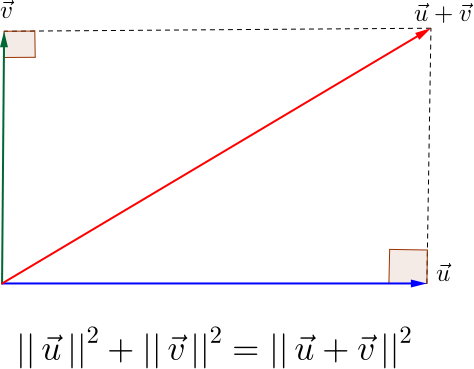
\includegraphics[scale=0.5]{pythagoras.png}
\end{center}
% section pythagoras_sats (end)

\section{Pythagoras sats i $\mathbb{R}^n$} % (fold)
\label{sec:pythagoras_sats_i_}
\begin{sats}
    Två vektorer i $\vec{u}$ och $\vec{v}$ är ortogonala om:
\[
    \norm{\vec{u} + \vec{v}}^2 = \norm{\vec{u}}^2 + \norm{\vec{v}}^2
\]

\end{sats}
\begin{bevis}
	\[
	    \norm{\vec{u} + \vec{v}}^2 = (\vec{u} + \vec{v}) \cdot (\vec{u} + \vec{v})
	\]
	Använd räkneregler för skalärprodukten:
	\begin{align*}
	&= (\vec{u} + \vec{v}) \cdot \vec{u} + (\vec{u} + \vec{v}) \cdot \vec{v} \\
	&= \vec{u} \cdot \vec{u} + \vec{v} \cdot \vec{u} + \vec{u} \cdot \vec{v} + \vec{v} \cdot \vec{v} \\
	&= \norm{\vec{u}}^2+ 2(\vec{u} \cdot \vec{v}) + \norm{\vec{v}}^2
	\end{align*}
	dvs:
	\[
	    \norm{\vec{u} + \vec{v}}^2 = \norm{\vec{u}}^2 + \norm{\vec{v}}^2
	\]
	omm $\vec{u} \cdot \vec{v} = 0$, dvs $\vec{u}$ och $\vec{v}$ \underline{ortogonala}
\end{bevis}
% section pythagoras_sats_i_ (end)

\section{Linjärkombinationer i $\mathbb{R}^n$} % (fold)
\label{sec:linj_rkombinationer_i_}
En linjärkombination av vektorerna $\vec{v}_1, \vec{v}_2, \cdots, \vec{v}_n$ i $\mathbb{R}^n$ med vikterna $a_1, a_2, \cdots, a_n$ är vektorn:
\[
    \vec{v} = a_1 \cdot \vec{v}_1 + a_2 \cdot \vec{v}_2 + \cdots + a_n \cdot \vec{v}_n
\]
Standardbasen för $\mathbb{R}^n$ består av:
\begin{align*}
&&\vec{e}_1 = \begin{bmatrix} 1\\0\\\vdots\\0 \end{bmatrix}
&&&\vec{e}_2 = \begin{bmatrix} 0\\1\\\vdots\\0 \end{bmatrix}
&&&&\cdots
&&&&\vec{e}_n = \begin{bmatrix} 0\\0\\\vdots\\1 \end{bmatrix}
\end{align*}
Alla vektorer $\vec{v} \in \mathbb{R}^n$ kan skrivas som en linjärkombination av $\vec{e}_1, \vec{e}_2, \cdots, \vec{e}_n$:
\[
    \vec{v} = v_1 \cdot \vec{e}_1 + v_2 \cdot \vec{e}_2 + \cdots + v_n \cdot \vec{e}_n
\]
\begin{Ex}
    \begin{gather*}
    \vec{v} = \begin{bmatrix} 1\\2\\3\\5 \end{bmatrix} = 1 \cdot \begin{bmatrix} 1\\0\\0\\0 \end{bmatrix} + 2 \cdot \begin{bmatrix} 0\\1\\0\\0 \end{bmatrix} + 3 \cdot \begin{bmatrix} 0\\0\\1\\0 \end{bmatrix} + 5 \cdot \begin{bmatrix} 0\\0\\0\\1 \end{bmatrix}
    \end{gather*}
\end{Ex}
% section linj_rkombinationer_i_ (end)

\section{Matriser av godtycklig storlek} % (fold)
\label{sec:matriser_av_godtycklig_storlek}
Se föreläsning 5
% section matriser_av_godtycklig_storlek (end)

\section{Linjära avbildningar i $\mathbb{R}^n$} % (fold)
\label{sec:linj_ra_avbildningar_i_}
Om avbildningen $f:\mathbb{R}^n \rightarrow \mathbb{R}^m$ är en linjär avbildning så finns det en entydigt bestämd matris \textbf{A} sådan att:
\[
    f(\vec{x}) = \mathbf{A} \cdot \vec{x}
\]
\textbf{A} kallas standardmatrisen för avbildningen \textit{f} och bestäms av:
\[
    \mathbf{A} = \begin{bmatrix} f(\vec{e}_1)&f(\vec{e}_2)&\cdots&f(\vec{e}_n) \end{bmatrix}
\]
\begin{bevis}
	(följer direkt av att \textit{f} är linjär, se föreläsning 5)
	\begin{align*}
	f(\vec{x}) &= f(\overbrace{x_1 \cdot \vec{e}_1 + x_2 \cdot \vec{e}_2 + \cdots + x_n \cdot \vec{e}_n}^\text{ty \textit{f} linjär}) = x_1 \cdot f(\vec{e}_1) + x_2 \cdot f(\vec{e}_2) + \cdots + x_n \cdot f(\vec{e}_n) \\
	&= \overbrace{\begin{bmatrix} f(\vec{e}_1)&f(\vec{e_2})&\cdots&f(\vec{e}_n) \end{bmatrix}}^\text{\textbf{A}} \begin{bmatrix} x_1\\x_2\\\vdots\\x_n \end{bmatrix} = \mathbf{A} \cdot \vec{x}
	\end{align*}
	
\end{bevis}
Vi har en linje \textit{L}: $\vec{p} + t \cdot \vec{v}$
\begin{align*}
&\overbrace{\begin{bmatrix} p_1\\p_2\\\vdots\\p_n \end{bmatrix}}^\text{En punkt} + \overbrace{t}^\text{Ett tal} \cdot \overbrace{\begin{bmatrix} v_1\\v_2\\\vdots\\v_n \end{bmatrix}}^\text{Riktningsvektor}
\\
\end{align*}
\begin{center}
	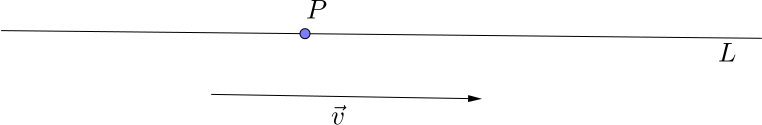
\includegraphics[scale=0.5]{lineandvector.png}
\end{center}
Låt en ortogonal projektion av $\vec{x}$ på \textit{L} vara $\vec{x}_L$, $\vec{x}_L$ är parallell med $\vec{v}$, så vi kan skriva:
\[
    \vec{x}_L = c \cdot \vec{v}
\]
och att ($\vec{x} - \vec{x}_L$) är ortogonal mot $\vec{v}$
\begin{center}
	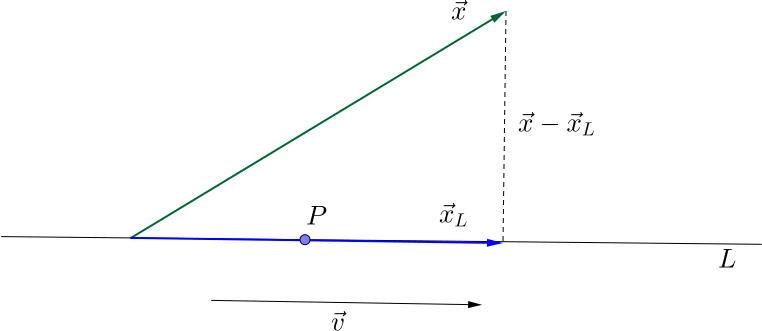
\includegraphics[scale=0.5]{projektion.png}
\end{center}
Formulera en linjär avbildning:
\begin{align*}
&f: \mathbb{R}^n \rightarrow \mathbb{R}^m
&& \mbox{ sådan att }
&&& \vec{x}_L = \mathbf{A} \cdot \vec{x}
\end{align*}
\textbf{Lösning}:\\
Vi vet att:
\begin{align*}
0 &= (\vec{x} - \vec{x}_L) \cdot \vec{v} \\
&= (\vec{x} - (c \cdot \vec{v})) \cdot \vec{v} \\
&= \vec{x} \cdot \vec{v} - c \cdot (\vec{v} \cdot \vec{v})
\end{align*}
Lös ut \textit{c}:
\[
    c = \frac{\vec{x} \cdot \vec{v}}{\vec{v} \cdot \vec{v}}
\]
Eftersom $\vec{x}_L = c \cdot \vec{v}$, får vi:
\begin{align*}
\vec{x}_L &= \frac{\vec{x} \cdot \vec{v}}{\vec{v} \cdot \vec{v}} \cdot \vec{v}\\
&= \frac{1}{\norm{\vec{v}}^2} \cdot (\vec{x} \cdot \vec{v}) \cdot \vec{v} \\
&= \frac{1}{\norm{\vec{v}}^2} \cdot \vec{v} \cdot (\vec{x} \cdot \vec{v}) \\
&= \frac{1}{\norm{\vec{v}}^2} \cdot \vec{v} \cdot (\vec{v} \cdot \vec{x}) \\
&= \frac{1}{\norm{\vec{v}}^2} \cdot \vec{v} \cdot \vec{v}^T \cdot \vec{x}
\end{align*}
\begin{Rem}
    Kom ihåg definitionen av skalärprodukt:
    \[
        \vec{x} \cdot \vec{y} = \begin{bmatrix} x_1, \cdots, x_n \end{bmatrix}\begin{bmatrix} y_1\\\vdots\\y_n \end{bmatrix} = \vec{x}^T \cdot \vec{y}
    \]
\end{Rem}
\[
    \vec{v} \cdot \vec{v}^T = \begin{bmatrix} v_1\\v_2\\\vdots\\v_n \end{bmatrix} \begin{bmatrix} v_1&v_2&\cdots&v_n \end{bmatrix} = 
    \begin{bmatrix} 
    v_1v_1 & v_1v_2 & \cdots & v_1v_n \\
    v_2v_1 & v_2v_2 & \cdots & v_2v_n \\
    \vdots & \vdots & \ddots & \vdots \\
    v_nv_1 & v_nv_2 & \cdots & v_nv_n
    \end{bmatrix}
\]
Låt:
\[
    \mathbf{A} = \frac{1}{\norm{\vec{v}}^2} \cdot \vec{v} \cdot \vec{v}^T
\]
då får vi:
\[
    f(\vec{x}) = \mathbf{A} \cdot \vec{x} \mbox{ } ( = \vec{x}_L)
\]
Ortogonalprojektionen är linjär och $\vec{x}_L = f(\vec{x})$ ges av:
\[
    \vec{x}_L = \frac{1}{\norm{\vec{v}}^2} \cdot \vec{v} \cdot \vec{v}^T \cdot \vec{x}
\]
% section linj_ra_avbildningar_i_ (end)
\end{document}